\subsection{Altering Human-AI collaboration dynamics}



% The current relationship between the AI and the human designer in EDD is one where the AI supports the designer in the form of presenting data in a helpful way, and enables the designer to easily apply the well curated high performing rooms through using PCG and MAP-Elites~\cite{p13MAP-Elites-eddy}. 
The standard version of EDD presents a unidirectional relationship between the human designer and the AI, where the AI can only suggest content adapted to the designer's room, called the target room. As concluded in Morai Maker~\cite{p13guzdial_co-creative_2018}, allowing the human designer and the computer-controlled agent to take turns in the creative process enables the possibility of an even influence between the co-creators; thus, the human user and the AI take turns placing down tiles. Here we present three modified versions of EDD that implement three different dynamics for the human-AI co-creative process. %(each version summarized in table~\ref{tab:AI-key-difference}).

% , where the human user and the AI will place down tiles in a turn based fashion.

% in ascending order of computer initiative:
% \begin{figure}
% \centering
%     \includegraphics[scale=0.4]{images/Artifact/EDD Flowchart.drawio.png}
%     \caption{Flowchart illustrating the flow of EDD.}
%     \label{fig:my_label}
% \end{figure}



\subsubsection{AI Version 1 (AIv1) - Low degree of agency} 

In this version the AI takes a suggestion colleague role. As the human manually designs a target room, the AI suggests tiles directly on top of the design. The human has the option to make use of the suggested tiles at will, placing them on the target room by clicking on them in the user interface. Both the human and the AI can override each other tiles.

%It takes a step further than 

%The human can overwrite any AI-authored tiles so that the computer does not have any influence on the end result.

%AI-suggested tiles that the human uses are registered as AI-authored tiles.

% , but it is more present in its suggestive role than it is in the standard version of EDD.

\subsubsection{AI Version 2 (AIv2) - Medium degree of agency} 

In this version, the AI places directly its recommended tiles rather than suggesting. Like in AIv1, both the human and the AI can override each other tiles.

%In this dynamic, the AI place down the tiles on their turn rather than suggesting, but the human has the option to overwrite them. This means that the end result can still be solely contributed by the human designer.

% However, the designer still has the option to overwrite the AI's contributions to the target room, meaning the end result can still be solely contributed by the human designer.

\subsubsection{AI Version 3 (AIv3) - High degree of agency} 

Unlike in the other versions, in AIv3, the human designer cannot be the sole contributor to the room designs. The AI places the tiles on their turn rather than suggesting, and the human cannot overwrite them. However, the AI can overwrite human tiles in their turn. This allows the exploration of how human designers react to being in a co-creative relationship where the AI has more control than them and add constraints to their design and goals.

% The human user and the AI will place down tiles in a turn based fashion. The human can not overwrite the tiles placed down by the AI. In this version, it is not possible for the human designer to be the sole contributor to the room designs. This version allows to explore how human designers react to being in a co-creative relationship where the AI has more control than the human, as the AI can overwrite the human's contributions, but the human can not overwrite the AI-placed tiles.

\begin{figure*}[]
 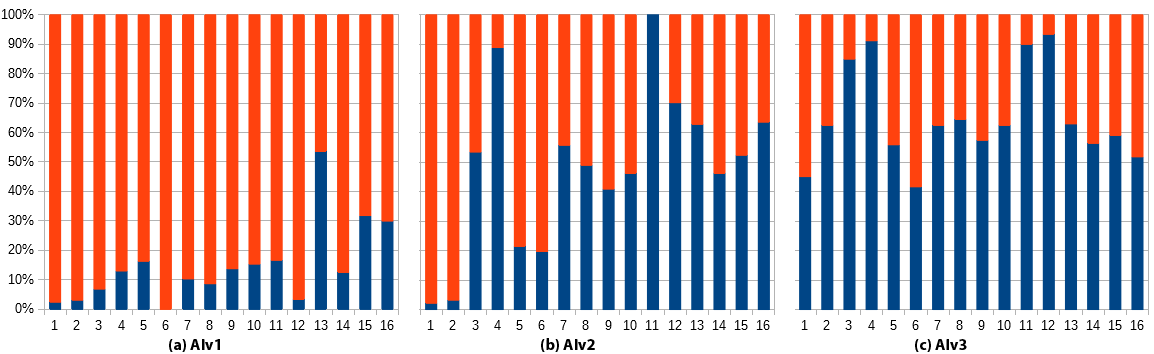
\includegraphics[width=\textwidth]{images/combined-bars.png}
 \caption{Percentage of tiles per co-creator in the rooms. Blue and Red bars relate to AI and Human placed tiles, respectively.}
 \label{fig:human-ai-contribution}
\end{figure*}

% \begin{figure}
%     \centering
%     \includegraphics[width=\columnwidth]{images/Artifact/Turns Flowchart.drawio.png}
%     \caption{The turn-based creative process.}
%     \label{fig:my_label}
% \end{figure}

\subsubsection{The Design of the AI}

%In future work, 

%This was shown to explore more of the space, but generate less performing individuals. However, combining both 

%We use all seven dimensions, which was shown to explore , which its adaptiveness to continuous editions, such as the ones done  was later assessed 

%The work in~\cite{p13alvarez_interactive_2020} shows

The goal is for the AI to be perceived as dynamic, responsive, and helpful but not totally predictable. These qualities were selected to try to create a co-creator that supports the design choices of the human but also introduces unexpected elements to stimulate lateral thinking. By making the AI dynamic and responsive, the aim is to minimize the risk of unsatisfactory asymmetric design between the AI and the human, as reported by~\cite{p13guzdial_co-creative_2018}, where some of the critiques mentioned that the AI was designing its own parts of the level instead of creating consistency with the human designer's contributions.

% \subsubsection{Limitations and variables}
% There are some limitations and rules that need to be implemented for the system to work well.
% Firstly, a limit to the amount of tiles the human designer places down during his turn needs to be implemented. This constraint is necessary for the sake of the two agents taking turn in the creation, and minimizing the risk of one agent being the sole contributor. 

For all three versions of the AI, the AI component creates and regularly updates a list of generated tiles. IC MAP-Elites constantly runs in the background, maintaining a list of elites across its seven dimensions. When the human ends their turn, the elites are processed by a KNN algorithm (K=20) that picks the set of tiles that will be used by the AI contributor comparing the elites to the target room on the seven dimensions. The resulting list of elites is further processed tile by tile, creating a final list that contains the most reoccurring tile types per position in the contribution area, which constitutes the list of generated tiles for the computer to use. From this list, and to further the perception of the AI being dynamic, it selects a random amount of tiles between 50\% and 100\% of the amount of human-placed tiles. However, through this process it is likely that the agent will not be human-like. For example, humans are likely to favor symmetry in a room, but the AI in this tool will consider all dimensions equal. The AI will also consider all types of tiles equally when calculating the most common tile in a position in the generated rooms.

%Through this process it is possible it will select a random amount of tiles between 50\% The AI contributes with what it determines to be the best tiles for the target room in the current contribution area using its methods of calculations, and it is likely that


Furthermore, depending on the level of agency, these tiles are just displayed as suggestions on the UI or directly placed when the computer takes control of the creative process. Both creators have a maximum of 12 tiles that they can contribute per turn. This was determined through experimentation during development since it is large enough to allow the designer to create a small subsection during their turn. If the human does not contribute one round before pressing "End Turn," the previous turn's amount of tiles are used for the calculation to enable the human to press "End Turn" repeatedly to let the AI keep contributing if that is desired. The available locations for the AI to contribute each turn are limited to a rectangular area surrounding the tiles the human designer recently placed, including a margin of 1 tile.

%To further the perception of the AI being dynamic, it contributes with a random amount of tiles between 50\% and 100\% of the amount of human-placed tiles.



% , including a margin of 1 tile. This choice is made to support a responsive and collaborative behavior of the AI that builds on the human designer's contribution.

% The margin for the contribution area is set to 1, as it was found during experimentation that any margin bigger than this is likely perceived as the AI contributing to other areas than the ones the human is focused on, because of the default size of the room being relatively small.

% As an example, if the human designer places down 8 tiles during his turn, the AI will contribute with 4-8 tiles, with the exact number being random within that range. The next turn the human designer might place down only 1 tile, and the AI will then respond with contributing 1 tile.

% The locations available for the AI to contribute in for each turn are limited to a rectangular area surrounding the tiles the human designer recently contributed with, including a margin of 1 tile. This choice is made to support a responsive and collaborative behavior of the AI that builds on the human designer's contribution.

% . If the AI where able to contribute with tiles all over the room, the AI will likely contribute with tiles at various locations in the room during one turn, and the human designer might perceive this as incoherent behaviour. 
% In Morai Maker~\cite{p13morai-maker}, the AI could place elements at any valid location in the level during its turn. One could argue that this is a possible cause of the criticism from the study's participants, regarding incoherent and disconnected contributions from the AI in relation to the human designer's creation.
% To counter this, the AI will contribute with tiles in

% . %not yet decided 
% The size of the margin was decided by experimentation.
% .



%\subsubsection{Determining the choice of tiles}



% The KNN algorithm receives the elites as the data, and the target room as the query, to find the K elites that are the closest to it, using the all of the seven dimensions included in EDD IC MAP-Elites \cite{p13MAP-Elites-eddy}. K is set to 20 through experimentation. This removes those elites that are far from what the designer is currently working with in the target room. 

% The resulting list of elites is further processed tile by tile, creating a final list that contains the most reoccurring tile-types per position in the contribution area, which constitutes the list of generated tiles for the computer to use.

% To determine what tiles to return in the list, a combination of techniques is used. The MAP-Elites algorithm runs continuously in the room editing view, on 50 procedurally generated rooms. When the MAP-Elites are done, they are saved in the AI-entity, and the algorithm can continue to run to optimize the elites further. When the button "End turn" is pressed, the saved elites are used by the AI to start calculating the contributions. This does mean that it is possible that the newest additions from the human designer was not considered in the MAP-Elites batch used to calculate the AI's contribution. Through experimentation while developing the artifact, a significant issue with efficiency was identified when the AI waited to run MAP-Elites with the new additions from the human every time it was its turn. The MAP-Elites algorithm need a few seconds to run, the time depending on how many rooms are generated. By lowering the amount of generated rooms significantly, the MAP-Elites would run faster, however decrease the quality of the elites too greatly to be a considerable compromise. Therefore, it was decided to continuously batch the MAP-Elites, and have the AI's turns being less complimentary of the human's additions.


% The elites are condensed by using a K-Nearest-Neighbour (KNN) algorithm. KNN works by finding the distances between a query and all the examples in the data, and return the specified number of examples (K) closest to the query. The number K is determined by experimentation, however deciding the best K value can be difficult, as a too high number K results in heavy averaging of all variables, while a too low number K results in bad categorizations. 
% The AI uses the KNN algorithm by giving the elites as the data, and the target room as the query, to find the K elites that are the closest to the target room, using the all of the seven dimensions.
% The value K that the AI uses is decided through experimentation to be 20. 
% The motivation of doing this, is to eliminate elites that are far from what the designer is currently working with in the target room. Additionally, the list of elites need to be condensed into a list with more relevant room suggestions, to avoid including rooms vastly different from the target room. 
% The next step is to use the elites to calculate the most reoccurring tile type for each position in the contribution area.
% If the elites are too varied in this step, all tiles will have an occurrence close to once, or zero, and there will not be any strong representation of tiles in any position. When using the resulting list of the KNN-algorithm, the tiles have larger differences in occurrences. Additionally, the rooms that the tiles are part of will likely have a higher chance to be a continuation of what the designer is attempting to create. 
% The AI now contributes with the resulting tiles of the highest occurrence, within the contribution area and amount of tiles to contribute with.


% \subsubsection{The General Behaviour of the AI}
% The resulting agent from the design choices is one that contributes with what it determines to be the best tiles for the target room in the current contribution area using its methods of calculations, and it is likely that this agent will not be human-like. For example, humans are likely to favor symmetry in a room, but the AI in this tool will consider all dimensions equal. The AI will also consider all types of tiles equally when calculating the most common tile in a position in the generated rooms. One could argue that humans do not consider all types of tiles equally, for example treasures or enemies are likely considered of higher value than floor-tiles, as they likely contribute more to valuable game design elements, such as challenge and reward.
% As the purpose of the study focuses on how the human designer reacts to the varying degrees of initiative and control of the AI, the behaviour and how the human designer gets along with the AI is of great importance. However, an AI that collaborates very well with the human designer is also less likely to bring forward valuable situations for this study, namely where the human is challenged and constrained. With these possible weaknesses of the behaviour of the AI in mind, the choice remains to keep the AI simple and calculated.


% \subsubsection{User Interface}
% The visual changes made to the program are all present in the room-editing view. In the room-editing view, an "End Turn"-button is now placed on the right of the target room, which ends the human designer's turn and starts the AI's turn when clicked. The map of MAP-Elites on the right side of the view is no longer visible. The buttons used for locks in the generation of new rooms is disabled. 
% All tiles placed by the AI will have a pink tint.

% When AIv1 is active, and it is the AI's turn to contribute, the clickable suggested tiles are displayed with a green tint directly on the target room, and a "Continue"-button will be displayed that when pressed, the suggestions are no longer displayed and it is the human's turn again. 

% \begin{figure}
%     \includegraphics[width=\columnwidth]{images/Artifact/both_tiles_arti.png}
%     \caption{Pink tinted tiles are placed by the AI, green tinted tiles are current suggestions.}
% \end{figure}

